\subsection{From the Conceptual Model to the Editor}
\label{subsec:art-editor-from-conceptual}

Basing our study on the XRM Conceptual Model (XRM) in \autoref{ch:conceptual-model} we adapted and modified it to suit a user-friendly and interactive modelling paradigm that would satisfy Fifthingenium's company needs and requirements of the component to implement.

Starting from the first part of the XRM, the Structural Model (\autoref{sec:conceptual-structural}), we decided to include as elements of the Editor only the fourth and, mostly, fifth level of abstraction (\autoref{fig:Legend}) of Non-Human Actors, as they represent a concrete category of assets that the editor can manage. Hence, the elements available in the Editor are: the \textit{QR Code} as only Interaction Placeholder element, \textit{Static 3D Model}, \textit{Text}, \textit{Image}, \textit{Dynamic 3D Model} and \textit{Video} (respectively referred to as \textit{3D Video} and \textit{2D Video}), \textit{Menu} and the \textit{360° Video} and \textit{3D Scene} as Environments. The Environemnt, differently from XRM, is not dependent on the technology but is referred as a sub-part of the Environment or a container of the objects and areas in it.
\begin{table}[h]
\centering
\begin{tabular}{|l|r|}
\hline
\textbf{XRM Actors}             & \textbf{ART Editor Elements} \\ \hline
QR Code                & QR Code             \\ \hline
Static 3D Model        & 3D Model            \\ \hline
Text                   & 2D Text             \\ \hline
Image                  & 2D Image            \\ \hline
Dynamic 3D Model       & 3D Video            \\ \hline
Video                  & 2D Video            \\ \hline
Menu                   & Menu                \\ \hline
360° Video Environment & 360° Video          \\ \hline
\begin{tabular}[c]{@{}l@{}}Augmented Environment\\  Virtual Environment\end{tabular} & 3D Scene \\ \hline
\end{tabular}
\caption{Comparison of XRM Actors and ART Editor Elements}
\label{table:xrm-art-actors}
\end{table}

Compared to the Behavioural Model (\autoref{sec:conceptual-behavioral}), in the ART Editor the Human Actor is implicitly involved in each interaction, so it hasn't been included in the modelling environment. A design choice was not to show all Actors' properties in their editor's counterpart because some of them are bounded to the nature of the digital asset being uploaded -- therefore these properties are set during the assets upload phase -- others, instead, (e.g. 3D Scene's World Anchors, Virtual Objects' position and orientation) are set during the on-site authoring phase and setting these properties at this authoring level would add an additional layer of difficulty not in the scope of the ART Project. For these reasons we chose to represent the change of elements' structural properties using a 'decoration' approach, allowing to visualize the relevant changes of properties with "tag elements" attached to each element; the same notation has been adopted with the interactions, keeping the \gls{UI} coherent and organizing elements into state and action nodes.
A comparative example is presented in \autoref{fig:comparison-effect-xrm-art}, in which the effect of making a 3D Model visible in XRM (\autoref{fig:xrm-effect}) is represented as an additional Visible "tag" in ART Editor (\autoref{fig:art-effect}) that indicates the visibility property set to on, with an opacity value of 100\%.
\begin{figure}[h]
    \begin{subfigure}{0.5\textwidth}
        \centering
        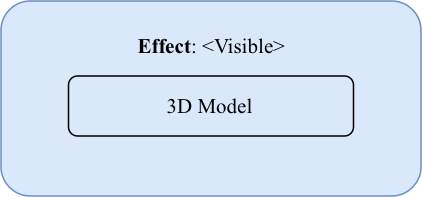
\includegraphics[width=\columnwidth]{Figures/Editor/xrm-effect.png}
        \caption{XRM Effect}
        \label{fig:xrm-effect}
    \end{subfigure}
    \begin{subfigure}{0.45\textwidth}
        \centering
        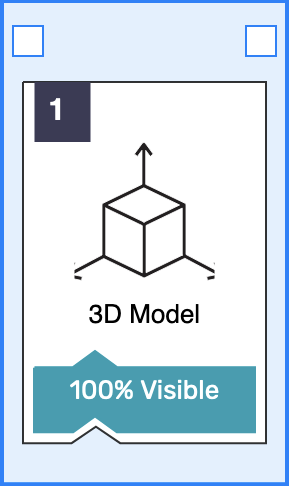
\includegraphics[width=0.5\textwidth]{Figures/Editor/art-effect.png}
        \caption{ART Editor State Tag}
        \label{fig:art-effect}
    \end{subfigure}
    \caption{Comparison of XRM Effect notation with ART Editor State Tag notation}
    \label{fig:comparison-effect-xrm-art}
\end{figure}

The concepts of Interaction and Task are derived from the Interaction Model (\autoref{sec:conceptual-interaction}): the former uses a structure very similar to the XRM (\autoref{fig:xrm-interaction}), adding user actions as "action tags" to the target (\autoref{fig:art-action}) in nodes called Action that can contain more than one interaction performed at the same time; finally, a Task in ART is implemented in the editor as a link between an Action and the corresponding effects -- namely, a State including the target elements with their appropriate tags representing a change of structural properties (\autoref{fig:comparison-task-xrm-art}).
\begin{figure}[h]
    \begin{subfigure}{0.5\textwidth}
        \centering
        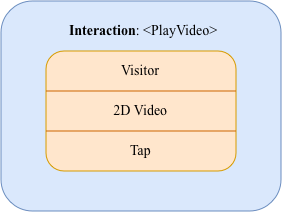
\includegraphics[width=0.85\columnwidth]{Figures/Editor/xrm-interaction.png}
        \caption{XRM Interaction}
        \label{fig:xrm-interaction}
    \end{subfigure}
    \begin{subfigure}{0.45\textwidth}
        \centering
        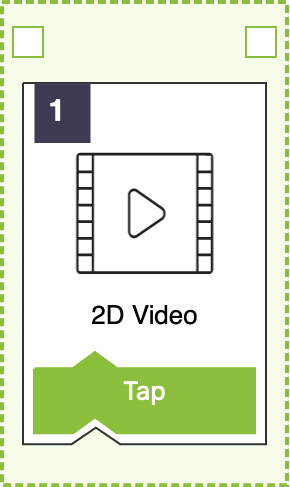
\includegraphics[width=0.5\textwidth]{Figures/Editor/art-action.png}
        \caption{ART Editor Action}
        \label{fig:art-action}
    \end{subfigure}
    \caption{Comparison of XRM Interaction with ART Editor Action}
    \label{fig:comparison-action-xrm-art}
\end{figure}

\begin{figure}[H]
    \begin{subfigure}{\textwidth}
        \centering
        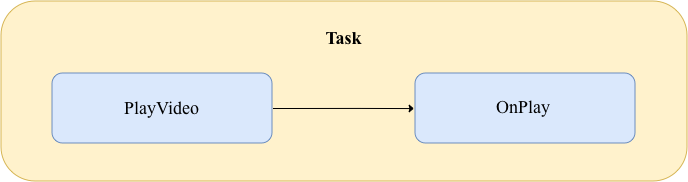
\includegraphics[width=0.7\columnwidth]{Figures/Editor/xrm-task.png}
        \caption{XRM Task}
        \label{fig:xrm-task}
    \end{subfigure}
    \begin{subfigure}{\textwidth}
        \centering
        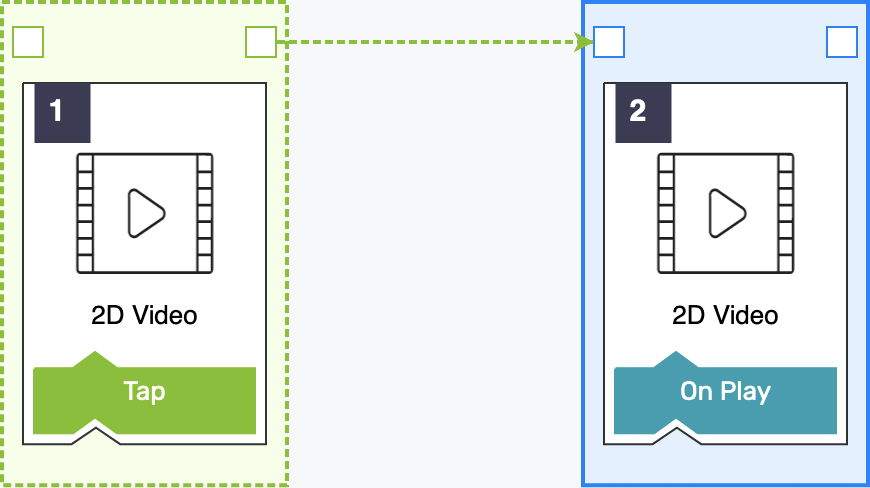
\includegraphics[width=0.7\columnwidth]{Figures/Editor/art-task.png}
        \caption{ART Editor Task}
        \label{fig:art-task}
    \end{subfigure}
    \caption{Comparison of XRM Task with ART Editor Task}
    \label{fig:comparison-task-xrm-art}
\end{figure}